It has been just been shown that the signals in Figure \ref{fig:feyn} are phenomenologically well motivated from the stand point of the \BL MSSM, as well as motivated experimentally in so far as it is possible with physical intuition and cross section calculations.
We are now effectively invited to start to design the search strategy.
It is very much worth noting that at this logical stage in the analysis the signal is further motivated by way of \emph{sensitivity studies}. 
These are studies done using a simplified version of the analysis done on quickly generated simulated samples.
This allows for a much more detailed assessment of signal sensitivity beyond cross section calculations.
This is also a necessary requirement, and an important part of the process, for requesting official simulated data in the ATLAS collaboration. 
%This is done to see if the signal would be seen against the background using an the complex kinematics that are present in events. 
These studies will not be detailed here as their development are almost entirely contained in the full search strategy.
It suffices to say that these studies showed that the expected sensitivity was very much large enough to not be deterred from this search in any way, and to actually be very much excited about in every way.

\subsection{Signal}
\label{sec:strategy:signal}
The strategy for this search revolves around being able to fully reconstruct the mass of the \chone from its decay into a final state of three leptons, \triLepDecay.
This points to the main discriminating variable, \mZl, defined as the invariant mass of the leptonically decaying \Zboson\ boson and the associated direct-lepton\footnote{lepton directly from the decay of the \chono}.
Note that for the leptonic \Zboson\ boson decay, we shift the measured dilepton invariant mass to the \Zboson\ pole mass in order to reduce resolution effects.
We redefine \mZl as 
\begin{equation}
    m_{Z\ell} : m_{Z\ell} - m_{Z} + 91.2 ~GeV
    \label{eq:mzl}
\end{equation}
Where $\ell$ here refers to only light leptons (electrons and muons) as we will not endeavour to reconstruct taus in this search. 
%\subsubsection{Possible Vertices}
It is interesting to note here that when looking for terms in the \BL MSSM Lagrangian that can lead to \chono decays into SM particles that the term that is proportional to the photon exactly cancel.
That is to say that the decay \chone$\rightarrow\gamma\ell$ vanishes.
This leaves decays that involve only the massive gauge bosons and the \Higgs and an associated direct-lepton (charged or neutral) to consider.
Considering both chargino-pair and chargino-neutralino production, Table~\ref{tab:finalstates} shows the final states of interest that have at least one trilepton resonance from the chargino decay.
The analysis regions will be defined later in this chapter.
We also remain sensitive to other decays which may result in a leptonically decaying \Zboson\ later in the decay chain, e.g. when the \Higgs goes to \ZZ in \CCsignal\ $\rightarrow$\Hl\Hl.

%The initial selection of events (trigger level single )


%Since this is first and foremost a trilepton resonance search the latter category is defined as events which have exactly three light leptons. 
%\footnote{This analysis does not attempt to reconstruct \Wboson's and this stage in the decay chain}

%\CCsignal$\rightarrow$\Hl\Hl$\rightarrow$\ZZ$\ell$\Hl$\rightarrow\ell\ell$\Zboson$\ell$\Hl. 
%one in which we will optimize the signal sensitivity to and ultimately do a multi bin fit described in \ref{sec:stats}. 

\renewcommand{\arraystretch}{1.7}
\begin{table}[t]
\footnotesize
\centering{
\caption{Table of final states with a trilepton resonance from the chargino decay.
Separate selection algorithms (two-leg or one-leg) are designed for final states where both or only one of the supersymmetric particles can be fully reconstructed from the detected particles.
}
  \label{tab:finalstates}
  \begin{tabular*}{0.463\textwidth}{c | c | l | l}
  \toprule
    \multirow{2}{*}{Algorithm} & \multirow{2}{*}{Production}    &  \multirow{2}{*}{Decay} & \multirow{2}{*}{Final State} \\
    & & &  \\
    \hline
    \hline
    \multirow{4}{*}{Two Leg} & \multirow{3}{*}{\CCsignal}    & \multirow{2}{*}{\Zl\Zl} & \triLep \triLep       \\
            &              &        & \triLep \jj$\ell$        \\
    \cline{3-4}
            &              & \Zl\Hl & \triLep \bbbar$\ell$    \\
    \cline{2-4}
            & \CNsignal    & \Zl\Wl & \triLep \jj$\ell$        \\
  \bottomrule
     \multirow{6}{*}{One Leg} &  \multirow{3}{*}{\CCsignal}    & \Zl\Zl & \triLep $\nu\nu\ell$       \\
    \cline{3-4}
            &              & \Zl\Hl & \triLep \WW$\ell$     \\
    \cline{3-4}
            &              & \Zl\Wv & \triLep \jj$\nu$       \\
    \cline{2-4}
            &  \multirow{3}{*}{\CNsignal}    & \Zl\Zv & \triLep \jj$\nu$       \\
    \cline{3-4}
            &              & \Zl\Hv & \triLep \WW$\nu$       \\
    \cline{3-4}
            &              & \Zl\Wl & \triLep $\ell\nu\ell$        \\
  \bottomrule
  \end{tabular*}
}
\end{table}

\subsection{Backgrounds}
\label{sec:strategy:background}
The SM processes that are expected to contribute largely to this signal's background are those that produce many leptons and contain a Z boson, these processes include \WZ, \ZZ, and \ttZ.
Figure \ref{fig:SMxs} shows a summary of several SM total and fiducial cross section measurements from \atlas for four center-of-mass energies, \rts, as well as their corresponding theoretical expectations. 
From this figure what is immediately obvious is all the very large backgrounds that, naively, we should not expect to have to deal with based on the the assumptions just made.
i.e. we shouldn't expect large contributions from any process to the left of \VV in Figure \ref{fig:SMxs}.
This assumption is of course built on absolute truth knowledge of all the SM processes final states and we will later see that this is not a very good assumption for a particular background. 
The strategy for handling these backgrounds in order to accurately estimate their yields in the signal regions in which we intend to make a statement about take on this particular form: \emph{small} backgrounds will be directly estimated with Monte Carlo.
The dominant backgrounds, \WZ, \ZZ, and \ttZ will be estimated with dedicated control regions, to be described in detail in Sections~\ref{sec:crwz}, to~\ref{sec:crttz}, by way of data-MC normalization parameters for those background signatures contained in the full statistical fit that will be described in Section \ref{sec:stats}.
The corrected estimation is then validated in dedicated validation regions before being propagated to the signal regions. 
The contribution from events with one or more misidentified or nonprompt (fake) leptons is separately estimated using a data-driven method to be described in Section~\ref{sec:fakes}.

\begin{figure}[tbp]
  \begin{center}
    %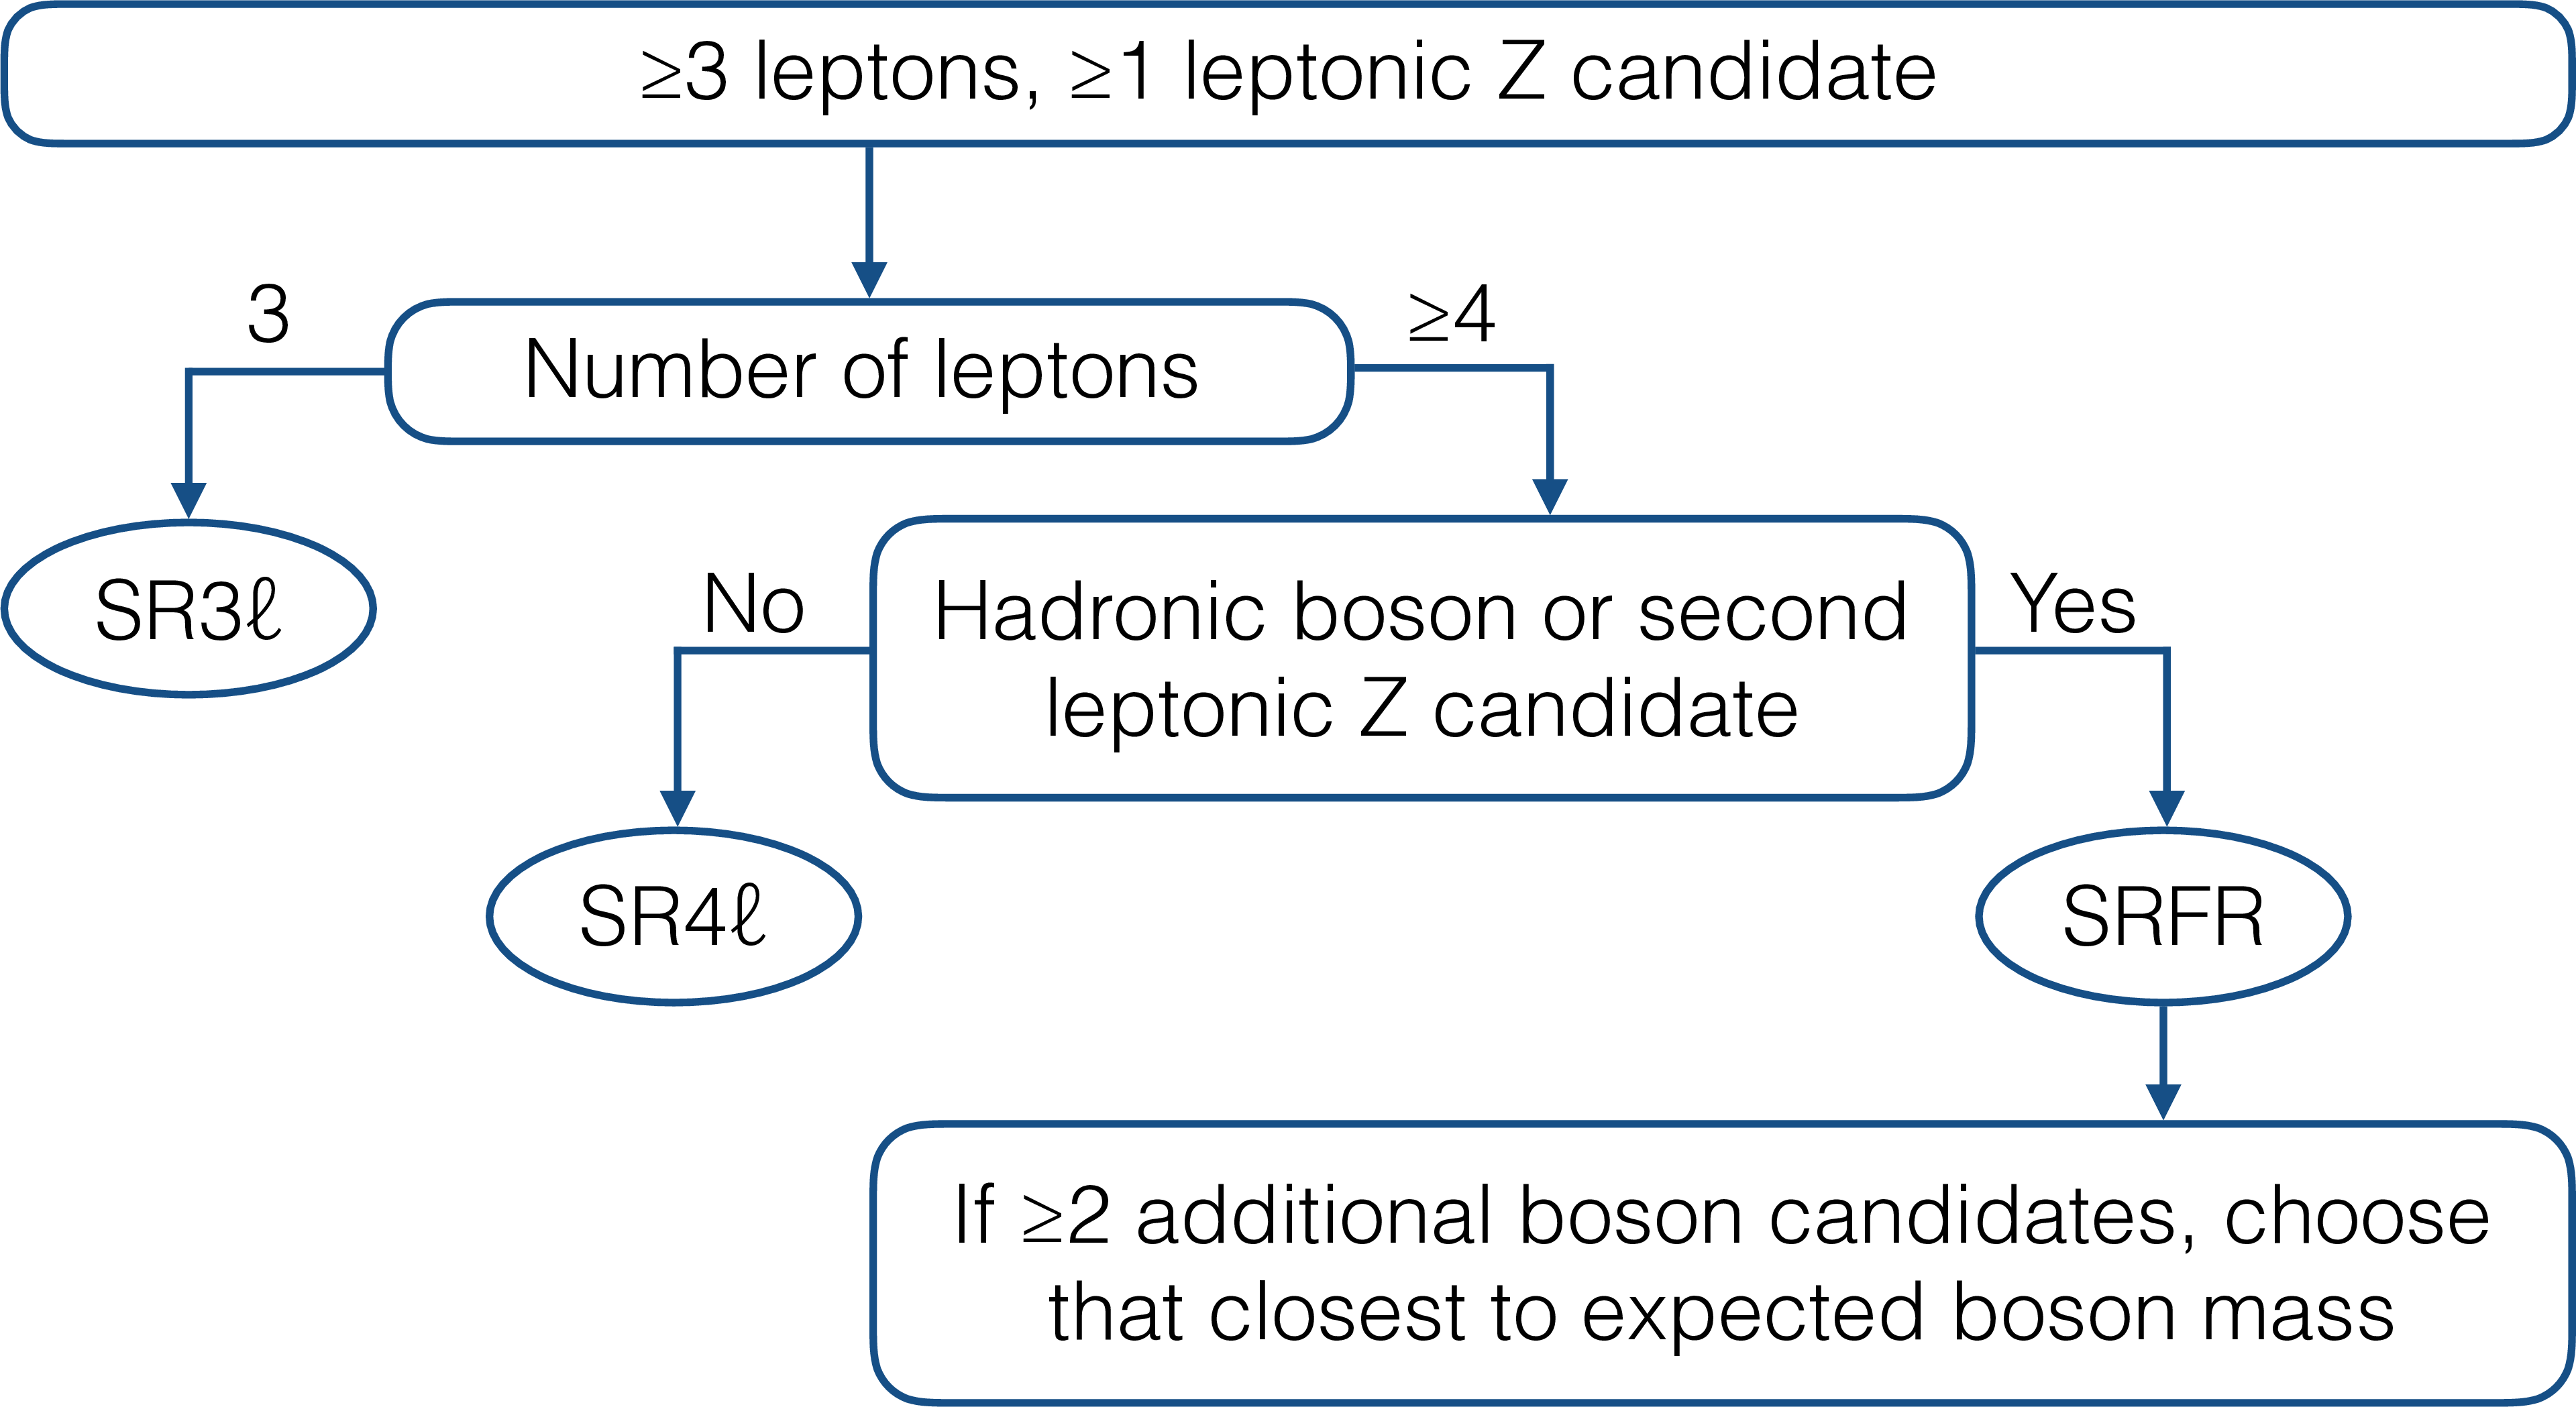
\includegraphics[width=0.98\textwidth]{figs/rpvthreel/3LRPVSchematic.pdf}
    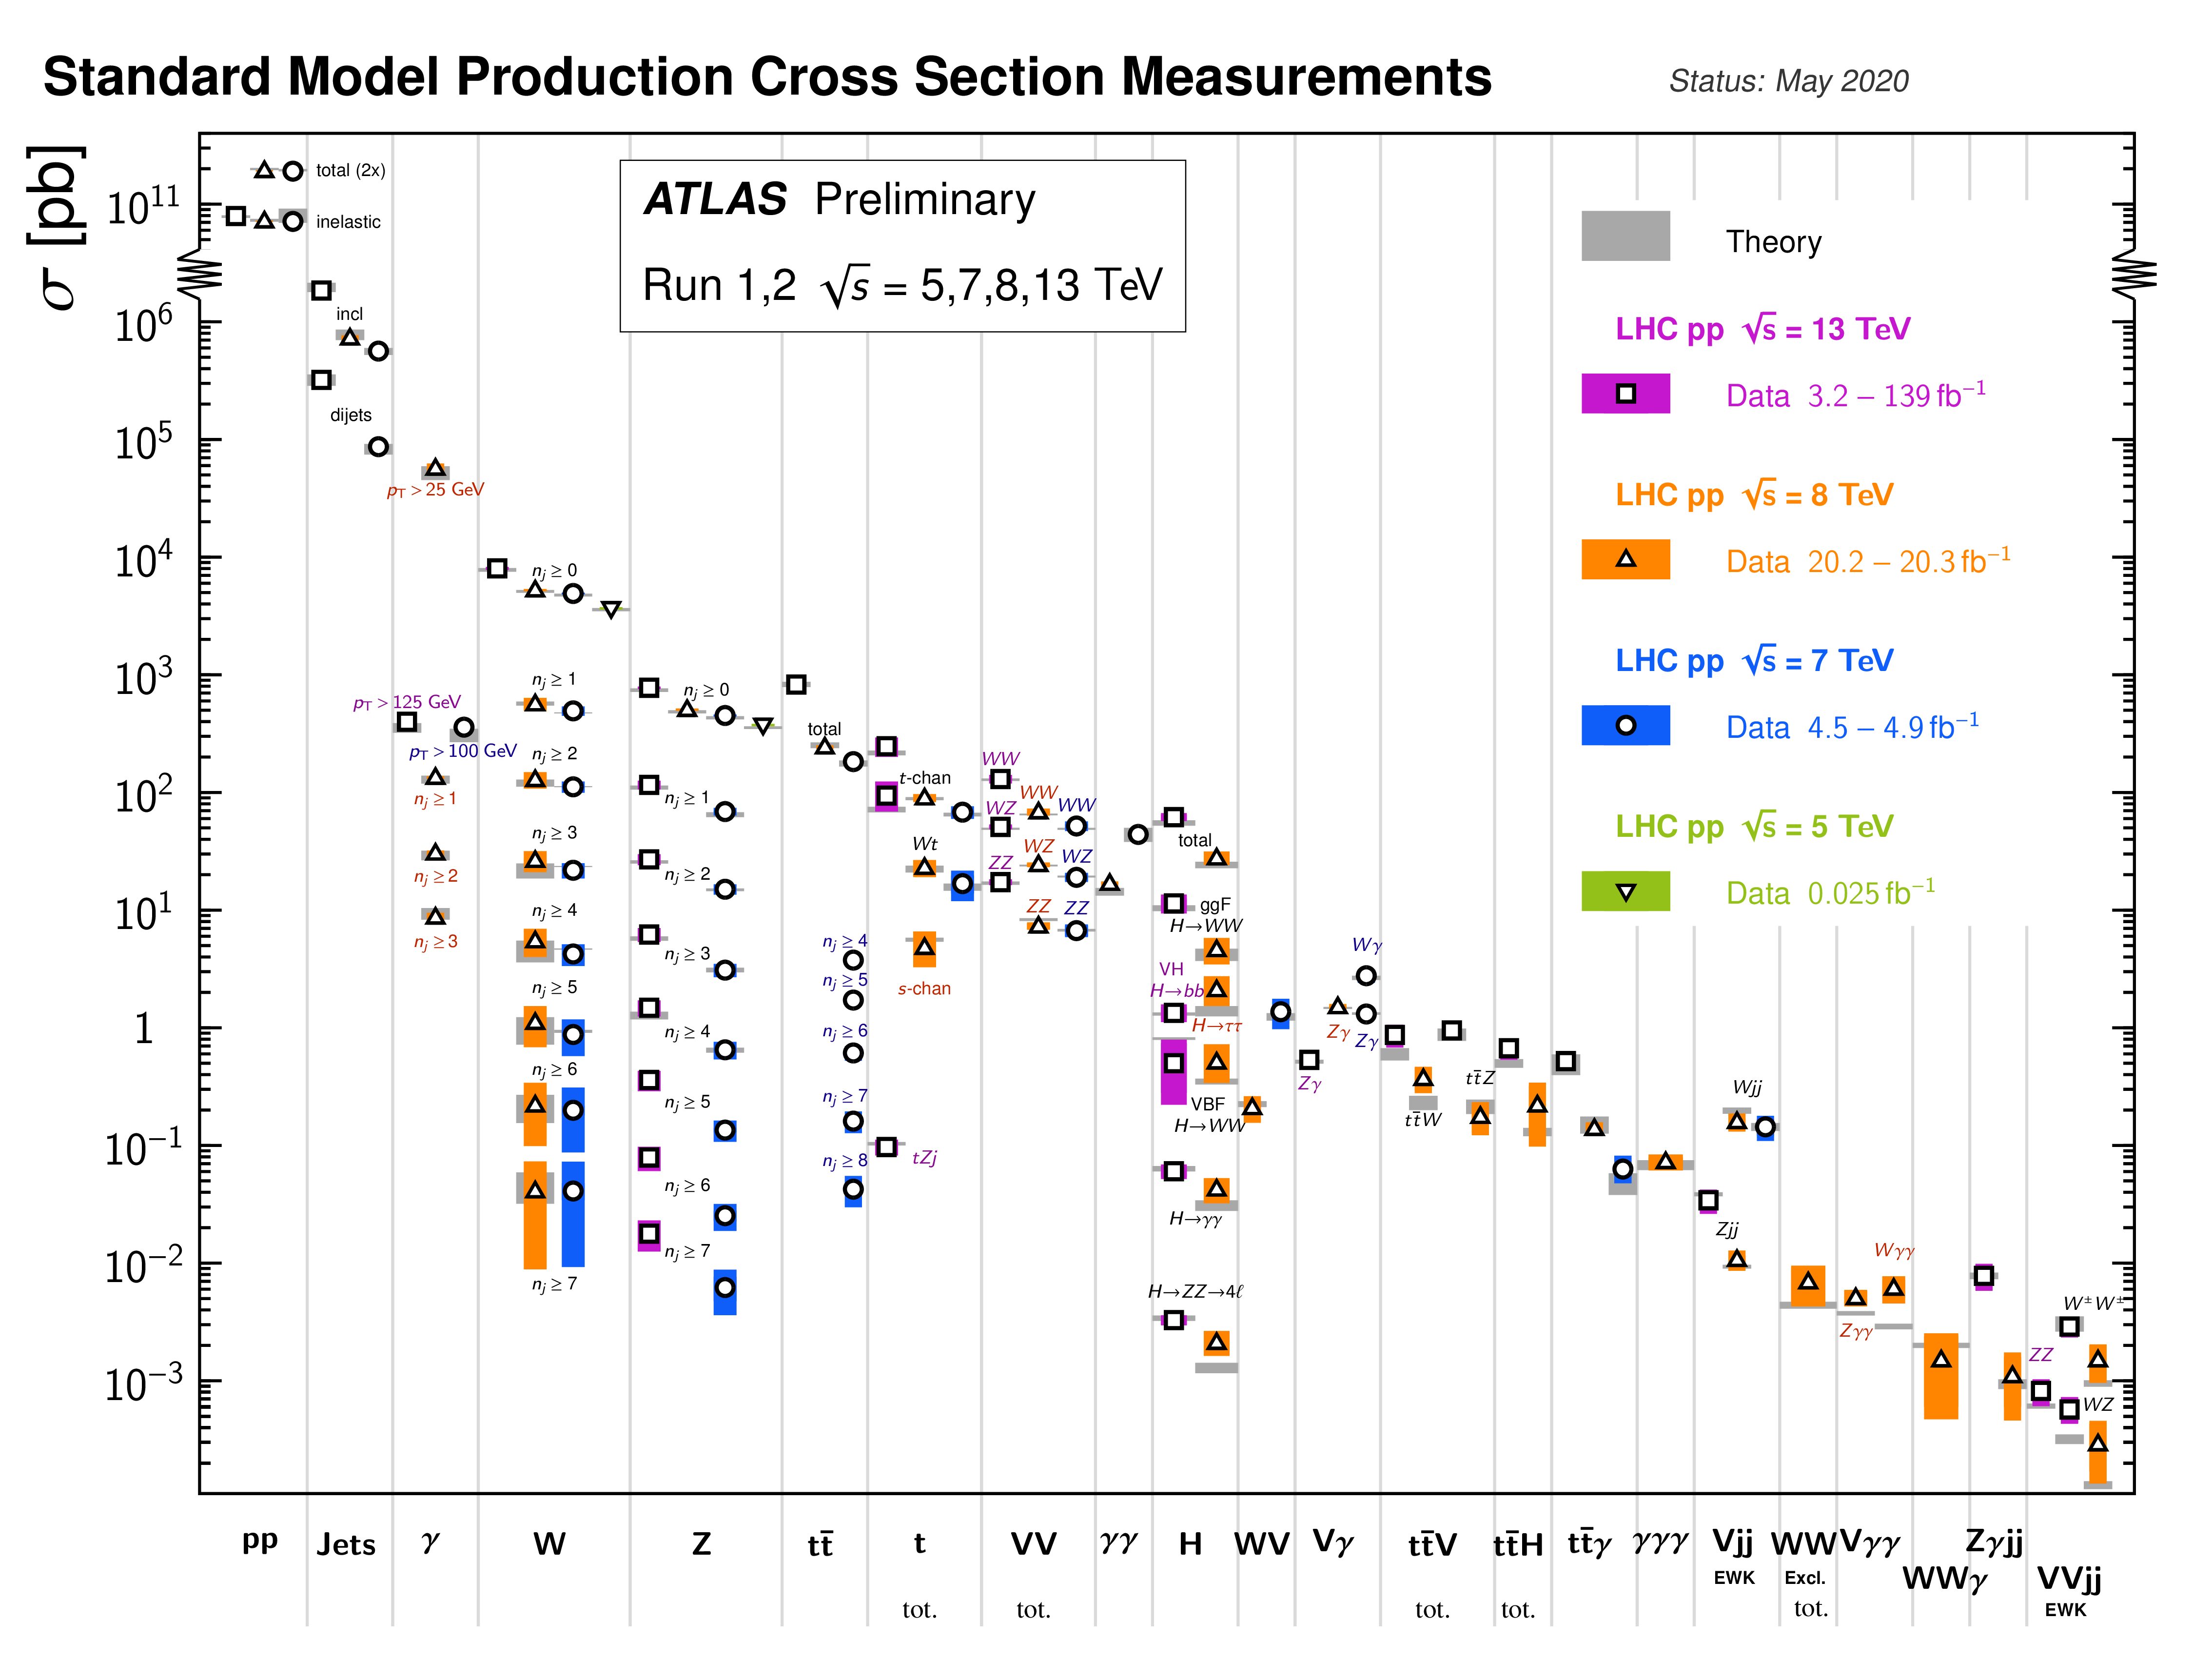
\includegraphics[width=0.99\textwidth]{figs/rpvthreel/SMcrossSections.png}
  \end{center}
  \caption[Summary of several Standard Model total and fiducial production cross section measurements, corrected for branching fractions, compared to the corresponding theoretical expectations.]
          {Summary of several Standard Model total and fiducial production cross section measurements, corrected for branching fractions, compared to the corresponding theoretical expectations. In some cases, the fiducial selection is different between measurements in the same final state for different centre-of-mass energies \rts, resulting in lower cross section values at higher \rts \cite{ATL-PHYS-PUB-2020-010}.}
   \label{fig:SMxs}
\end{figure}


%\textbf{\textcolor{red}{$\rightarrow$ }}\\